%%%%%%%%%%%%%%%%%%%%%%%%%%%%%%%%%%%%%%%%%
% Classicthesis Typographic Thesis
% LaTeX Template
% Version 1.3 (15/2/14)
%
% This template has been downloaded from:
% http://www.LaTeXTemplates.com
%
% Original author:
% André Miede (http://www.miede.de)
%
% License:
% CC BY-NC-SA 3.0 (http://creativecommons.org/licenses/by-nc-sa/3.0/)
%
% General Tips:
% 1) Make sure to edit the classicthesis-config.file
% 2) New enumeration (A., B., C., etc in small caps): \begin{aenumerate} \end{aenumerate}
% 3) For margin notes: \marginpar or \graffito{}
% 4) Do not use bold fonts in this style, it is designed around them
% 5) Use tables as in the examples
% 6) See classicthesis-preamble.sty for useful commands
%
%%%%%%%%%%%%%%%%%%%%%%%%%%%%%%%%%%%%%%%%%

%----------------------------------------------------------------------------------------
%	PACKAGES AND OTHER DOCUMENT CONFIGURATIONS
%----------------------------------------------------------------------------------------

\documentclass[
		twoside,openright,titlepage,numbers=noenddot,headinclude,1headlines,
                footinclude=true,cleardoublepage=empty,
                BCOR=5mm,paper=a4,fontsize=11pt, % Binding correction, paper type
                american, % Languages
                ]{scrreprt}

% Includes the file which contains all the document configurations and packages
% - make sure to edit this file

%%%%%%%%%%%%%%%%%%%%%%%%%%%%%%%%%%%%%%%%%
% Thesis Configuration File
%
% The main lines to change in this file are in the DOCUMENT VARIABLES
% section, the rest of the file is for advanced configuration.
%
%%%%%%%%%%%%%%%%%%%%%%%%%%%%%%%%%%%%%%%%%

%----------------------------------------------------------------------------------------
%	DOCUMENT VARIABLES
%	Fill in the lines below to enter your information into the thesis template
%	Each of the commands can be cited anywhere in the thesis
%----------------------------------------------------------------------------------------

% Remove drafting to get rid of the '[ Date - classicthesis version 4.0 ]' text
% at the bottom of every page
\PassOptionsToPackage{eulerchapternumbers, listings, drafting, pdfspacing,
subfig, beramono, eulermath, parts, dottedtoc, floatperchapter}{classicthesis}
% Available options: drafting parts nochapters linedheaders eulerchapternumbers
% beramono eulermath pdfspacing minionprospacing tocaligned dottedtoc
% manychapters listings floatperchapter subfig
% floatperchapter: numbering in equations, figures, etc per section
% Adding 'dottedtoc' will make page numbers in the table of contents flushed
% right with dots leading to them

\newcommand{\myTitle}{Small Area Estimation using Robust Area Level Models\xspace}
\newcommand{\mySubtitle}{Theory, Implementation, and Simulation Studies\xspace}
\newcommand{\myDegree}{Dr. rer. pol. (rerum politicarum)\xspace}
\newcommand{\myName}{Sebastian Warnholz\xspace}
\newcommand{\myProf}{Prof. Dr. Timo Schmid\xspace}
\newcommand{\myOtherProf}{Prof. Dr. Nikos Tzavidis\xspace}
\newcommand{\mySupervisor}{Put name here\xspace}
\newcommand{\myFaculty}{Fachbereich Wirtschaftswissenschaft\xspace}
\newcommand{\myDepartment}{Professur für Angewandte Statistik\xspace}
\newcommand{\myUni}{Freie Universitt Berlin\xspace}
\newcommand{\myLocation}{Berlin\xspace}
\newcommand{\myTime}{\today\xspace}
\newcommand{\myVersion}{version 0.7\xspace}

%----------------------------------------------------------------------------------------
%	USEFUL COMMANDS
%----------------------------------------------------------------------------------------

\newcommand{\ie}{i.\,e.}
\newcommand{\Ie}{I.\,e.}
\newcommand{\eg}{e.\,g.}
\newcommand{\Eg}{E.\,g.}

\newcounter{dummy} % Necessary for correct hyperlinks (to index, bib, etc.)
\providecommand{\mLyX}{L\kern-.1667em\lower.25em\hbox{Y}\kern-.125emX\@}

%----------------------------------------------------------------------------------------
%	PACKAGES
%----------------------------------------------------------------------------------------

\usepackage{hyphenat} % for \hyp hyphenation stuff

%------------------------------------------------

\usepackage{lipsum} % Used for inserting dummy 'Lorem ipsum' text into the template

%------------------------------------------------

\PassOptionsToPackage{utf8}{inputenc}
\usepackage{inputenc}

 %------------------------------------------------

\PassOptionsToPackage{british}{babel}  % Change this to your language(s)
% Spanish languages need extra options in order to work with this template
%\PassOptionsToPackage{spanish,es-lcroman}{babel}
\usepackage{babel}

%------------------------------------------------

%\PassOptionsToPackage{square,numbers}{natbib}
%\usepackage{natbib}
\usepackage[
natbib=true,
backend=biber,
style=authoryear, % author (2000)
maxcitenames=2,
maxbibnames=99,
uniquename=false
]{biblatex}
\addbibresource[datatype=bibtex]{Bibliography.bib}

 %------------------------------------------------

\PassOptionsToPackage{fleqn}{amsmath} % Math environments and more by the AMS
\usepackage{amsmath}
% \numberwithin{equation}{section}
\usepackage{mathtools}

 %------------------------------------------------

\PassOptionsToPackage{T1}{fontenc} % T2A for cyrillics
\usepackage{fontenc}

%------------------------------------------------

\usepackage{xspace} % To get the spacing after macros right

%------------------------------------------------

\usepackage{mparhack} % To get marginpar right

%------------------------------------------------

\usepackage{fixltx2e} % Fixes some LaTeX stuff

%------------------------------------------------

\PassOptionsToPackage{smaller}{acronym} % Include printonlyused in the first bracket to only show acronyms used in the text
\usepackage{acronym} % nice macros for handling all acronyms in the thesis

%------------------------------------------------

%\renewcommand*{\acsfont}[1]{\textssc{#1}} % For MinionPro
%\newcommand{\bflabel}[1]{{#1}\hfill} % Fix the list of acronyms

%------------------------------------------------

\PassOptionsToPackage{pdftex}{graphicx}
\usepackage{graphicx}

%----------------------------------------------------------------------------------------
%	FLOATS: TABLES, FIGURES AND CAPTIONS SETUP
%----------------------------------------------------------------------------------------

\usepackage{tabularx} % Better tables
\setlength{\extrarowheight}{2pt} % Increase table row height
\newcommand{\tableheadline}[1]{\multicolumn{1}{c}{\spacedlowsmallcaps{#1}}}
\newcommand{\myfloatalign}{\centering} % To be used with each float for alignment
\usepackage{caption}
\captionsetup{format=hang,font=small}
\usepackage{subfig}
% \usepackage[section]{placeins} % To keep floats within sections

%----------------------------------------------------------------------------------------
%	CODE LISTINGS SETUP
%----------------------------------------------------------------------------------------

\usepackage{listings}
%\lstset{emph={trueIndex,root},emphstyle=\color{BlueViolet}}%\underbar} % for special keywords
\lstset{language=[LaTeX]Tex, % Specify the language for listings here
keywordstyle=\color{RoyalBlue}, % Add \bfseries for bold
basicstyle=\small\ttfamily, % Makes listings a smaller font size and a different font
%identifierstyle=\color{NavyBlue}, % Color of text inside brackets
commentstyle=\color{Green}\ttfamily, % Color of comments
stringstyle=\rmfamily, % Font type to use for strings
numbers=left, % Change left to none to remove line numbers
numberstyle=\scriptsize, % Font size of the line numbers
stepnumber=5, % Increment of line numbers
numbersep=8pt, % Distance of line numbers from code listing
showstringspaces=false, % Sets whether spaces in strings should appear underlined
breaklines=true, % Force the code to stay in the confines of the listing box
%frameround=ftff, % Uncomment for rounded frame
frame=single, % Frame border - none/leftline/topline/bottomline/lines/single/shadowbox/L
belowcaptionskip=.75\baselineskip % Space after the "Listing #: Desciption" text and the listing box
}

%----------------------------------------------------------------------------------------
%	HYPERREFERENCES
%----------------------------------------------------------------------------------------

\PassOptionsToPackage{pdftex,hyperfootnotes=false,pdfpagelabels}{hyperref}
\usepackage{hyperref}  % backref linktocpage pagebackref
\pdfcompresslevel=9
\pdfadjustspacing=1

\hypersetup{
% Uncomment the line below to remove all links (to references, figures, tables, etc)
%draft,
colorlinks=true, linktocpage=true, pdfstartpage=3, pdfstartview=FitV,
% Uncomment the line below if you want to have black links (e.g. for printing black and white)
%colorlinks=false, linktocpage=false, pdfborder={0 0 0}, pdfstartpage=3, pdfstartview=FitV,
breaklinks=true, pdfpagemode=UseNone, pageanchor=true, pdfpagemode=UseOutlines,
plainpages=false, bookmarksnumbered, bookmarksopen=true, bookmarksopenlevel=1,
hypertexnames=true, pdfhighlight=/O, urlcolor=webbrown, linkcolor=RoyalBlue, citecolor=webgreen,
%------------------------------------------------
% PDF file meta-information
pdftitle={\myTitle},
pdfauthor={\textcopyright\ \myName, \myUni, \myFaculty},
pdfsubject={},
pdfkeywords={},
pdfcreator={pdfLaTeX},
pdfproducer={LaTeX with hyperref and classicthesis}
%------------------------------------------------
}

%----------------------------------------------------------------------------------------
%	BACKREFERENCES
%----------------------------------------------------------------------------------------

\usepackage{ifthen} % Allows the user of the \ifthenelse command
\newboolean{enable-backrefs} % Variable to enable backrefs in the bibliography
\setboolean{enable-backrefs}{false} % Variable value: true or false

\newcommand{\backrefnotcitedstring}{\relax} % (Not cited.)
\newcommand{\backrefcitedsinglestring}[1]{(Cited on page~#1.)}
\newcommand{\backrefcitedmultistring}[1]{(Cited on pages~#1.)}
\ifthenelse{\boolean{enable-backrefs}} % If backrefs were enabled
{
\PassOptionsToPackage{hyperpageref}{backref}
\usepackage{backref} % to be loaded after hyperref package
\renewcommand{\backreftwosep}{ and~} % separate 2 pages
\renewcommand{\backreflastsep}{, and~} % separate last of longer list
\renewcommand*{\backref}[1]{}  % disable standard
\renewcommand*{\backrefalt}[4]{% detailed backref
\ifcase #1
\backrefnotcitedstring
\or
\backrefcitedsinglestring{#2}
\else
\backrefcitedmultistring{#2}
\fi}
}{\relax}

%----------------------------------------------------------------------------------------
%	AUTOREFERENCES SETUP
%	Redefines how references in text are prefaced for different
%	languages (e.g. "Section 1.2" or "section 1.2")
%----------------------------------------------------------------------------------------

\makeatletter
\@ifpackageloaded{babel}
{
\addto\extrasamerican{
\renewcommand*{\figureautorefname}{Figure}
\renewcommand*{\tableautorefname}{Table}
\renewcommand*{\partautorefname}{Part}
\renewcommand*{\chapterautorefname}{Chapter}
\renewcommand*{\sectionautorefname}{Section}
\renewcommand*{\subsectionautorefname}{Section}
\renewcommand*{\subsubsectionautorefname}{Section}
}
\addto\extrasngerman{
\renewcommand*{\paragraphautorefname}{Absatz}
\renewcommand*{\subparagraphautorefname}{Unterabsatz}
\renewcommand*{\footnoteautorefname}{Fu\"snote}
\renewcommand*{\FancyVerbLineautorefname}{Zeile}
\renewcommand*{\theoremautorefname}{Theorem}
\renewcommand*{\appendixautorefname}{Anhang}
\renewcommand*{\equationautorefname}{Gleichung}
\renewcommand*{\itemautorefname}{Punkt}
}
\providecommand{\subfigureautorefname}{\figureautorefname} % Fix to getting autorefs for subfigures right
}{\relax}
\makeatother

%----------------------------------------------------------------------------------------

\usepackage{classicthesis}

%----------------------------------------------------------------------------------------
%	CHANGING TEXT AREA
%----------------------------------------------------------------------------------------

%\linespread{1.05} % a bit more for Palatino
%\areaset[current]{312pt}{761pt} % 686 (factor 2.2) + 33 head + 42 head \the\footskip
%\setlength{\marginparwidth}{7em}%
%\setlength{\marginparsep}{2em}%

%----------------------------------------------------------------------------------------
%	USING DIFFERENT FONTS
%----------------------------------------------------------------------------------------

% \usepackage[oldstylenums]{kpfonts} % oldstyle notextcomp
% \usepackage[osf]{libertine}
% \usepackage{hfoldsty} % Computer Modern with osf
% \usepackage[light,condensed,math]{iwona}
% \renewcommand{\sfdefault}{iwona}
% \usepackage{lmodern} % <-- no osf support :-(
% \usepackage[urw-garamond]{mathdesign} <-- no osf support :-(

% use upquote if available, for straight quotes in verbatim environments
\IfFileExists{upquote.sty}{\usepackage{upquote}}{}
% use microtype if available
\IfFileExists{microtype.sty}{\usepackage{microtype}}{}
\usepackage{biblatex}
\usepackage{color}
\usepackage{fancyvrb}
\newcommand{\VerbBar}{|}
\newcommand{\VERB}{\Verb[commandchars=\\\{\}]}
\DefineVerbatimEnvironment{Highlighting}{Verbatim}{commandchars=\\\{\},fontsize=\small}
% Add ',fontsize=\small' for more characters per line
\usepackage{framed}
\definecolor{shadecolor}{RGB}{248,248,248}
\newenvironment{Shaded}{\begin{snugshade}}{\end{snugshade}}
\newcommand{\KeywordTok}[1]{\textcolor[rgb]{0.13,0.29,0.53}{\textbf{{#1}}}}
\newcommand{\DataTypeTok}[1]{\textcolor[rgb]{0.13,0.29,0.53}{{#1}}}
\newcommand{\DecValTok}[1]{\textcolor[rgb]{0.00,0.00,0.81}{{#1}}}
\newcommand{\BaseNTok}[1]{\textcolor[rgb]{0.00,0.00,0.81}{{#1}}}
\newcommand{\FloatTok}[1]{\textcolor[rgb]{0.00,0.00,0.81}{{#1}}}
\newcommand{\CharTok}[1]{\textcolor[rgb]{0.31,0.60,0.02}{{#1}}}
\newcommand{\StringTok}[1]{\textcolor[rgb]{0.31,0.60,0.02}{{#1}}}
\newcommand{\CommentTok}[1]{\textcolor[rgb]{0.56,0.35,0.01}{\textit{{#1}}}}
\newcommand{\OtherTok}[1]{\textcolor[rgb]{0.56,0.35,0.01}{{#1}}}
\newcommand{\AlertTok}[1]{\textcolor[rgb]{0.94,0.16,0.16}{{#1}}}
\newcommand{\FunctionTok}[1]{\textcolor[rgb]{0.00,0.00,0.00}{{#1}}}
\newcommand{\RegionMarkerTok}[1]{{#1}}
\newcommand{\ErrorTok}[1]{\textbf{{#1}}}
\newcommand{\NormalTok}[1]{{#1}}

% prevent graphics from overflowing
\usepackage{graphicx}
\makeatletter
\def\maxwidth{\ifdim\Gin@nat@width>\linewidth\linewidth\else\Gin@nat@width\fi}
\def\maxheight{\ifdim\Gin@nat@height>\textheight\textheight\else\Gin@nat@height\fi}
\makeatother
\setkeys{Gin}{width=\maxwidth,height=\maxheight,keepaspectratio}

%%%%%%%%%% Version 1.0 %%%%%%%%%%

% Model:
% \newcommand{\nDomains}{D}
% \newcommand{\indexDomain}{i}
% \newcommand{\directStat}{y}
% \newcommand{\directStatIndexed}{y_{\indexDomain}}
% \newcommand{\trueStat}{\mu}
% \newcommand{\trueStatIndexed}{\mu_{\indexDomain}}
% \newcommand{\indexUnit}{j}
% \newcommand{\nUnitIndexed}{n_\indexDomain}

% Sampling-Error
% \newcommand{\samplingError}{e}
% \newcommand{\samplingErrorIndexed}{e_{\indexDomain}}
% \newcommand{\samplingErrorUnitIndexed}{e_{\indexDomain\indexUnit}}
% \newcommand{\samplingVariance}{\sigma_e^2}
% \newcommand{\samplingVarianceIndexed}{\sigma_{e, i}^2}
% \newcommand{\samplingSD}{\sigma_e}
%
% % Uni Error
% \newcommand{\unitError}{e}
%
% % Random Effects
% \newcommand{\randomEffectIndexed}{v_{\indexDomain}}
% \newcommand{\randomEffect}{v}
% \newcommand{\randomEffectVariance}{\sigma_v^2}
% \newcommand{\randomEffectSD}{\sigma_v}
% \newcommand{\RandomEffect}{\mathbf{v}}

% Regressors
% \newcommand{\xArea}{x_{\indexDomain}}
% \newcommand{\xUnit}{x_{\indexDomain\indexUnit}}
% \newcommand{\X}{\mathbf{X}}
% \newcommand{\indexRegressor}{p}
% \newcommand{\nRegressor}{P}

% Math Operators
% \DeclareMathOperator{\tr}{tr}
% \DeclareMathOperator{\diag}{diag}

% Matrix Notation
% \newcommand{\IdentityMatrix}{\mathbf{I}}


% Fixed Point
\newcommand{\aFH}{\psi(\mathbf{r})^\top \mathbf{U}^{\frac{1}{2}}\mathbf{V}^{-1}\frac{\partial\mathbf{V}}{\partial\theta}\mathbf{V}^{-1}\mathbf{U}^{\frac{1}{2}} \psi(\mathbf{r})}


%%%%%%%%%% Version 2.0 %%%%%%%%%%
% constants:

\newcommand{\sige}{\sigma_{e, i}^2}
\newcommand{\sigre}{\sigma_{u}^2}
\newcommand{\re}{u}

% funs:
\DeclareMathOperator{\tr}{tr}
\newcommand{\Tr}[1]{tr\left(#1\right)}
\DeclareMathOperator{\diag}{diag}
\newcommand{\Diag}[1]{diag\left(#1\right)}

% formats:
\newcommand{\Distr}[1]{\mathcal{#1}}
\newcommand{\mat}[1]{\mathbf{#1}}
\newcommand{\Exp}[1]{\mathbb{#1}}

% subscripts:
\newcommand{\si}[1]{#1_i}
\newcommand{\sij}[1]{#1_{ij}}

\newcommand{\textrrmse}{Boxplot with Relative Root Mean Squared Error (RRMSE)}
\newcommand{\textrbias}{Boxplot with Relative Bias (RBIAS)}


\begin{document}

\frenchspacing % Reduces space after periods to make text more compact

\raggedbottom % Makes all pages the height of the text on that page

\selectlanguage{american} % Select your default language - e.g. american or ngerman

%\renewcommand*{\bibname}{new name} % Uncomment to change the name of the bibliography
%\setbibpreamble{} % Uncomment to include a preamble to the bibliography - some text before the reference list starts

\pagenumbering{roman} % Roman page numbering prior to the start of the thesis content (i, ii, iii, etc)

\pagestyle{plain} % Suppress headers for the pre-content pages

%-------------------------------------------------------------------------------
%	PRE-CONTENT THESIS PAGES
%-------------------------------------------------------------------------------

% Title Page

\begin{titlepage}

\begin{addmargin}[-1cm]{-3cm}
\begin{center}
\large

\hfill
\vfill

\begingroup
\color{Maroon}\spacedallcaps{\myTitle} \\ \bigskip % Thesis title
\endgroup

\spacedlowsmallcaps{\myName} % Your name

\vfill

%
\includegraphics[width=6cm]{figs/FULogo_RGB} \\ \medskip % Picture

\mySubtitle \\ \medskip % Thesis subtitle
% \myDegree \\
% \myDepartment \\
% \myFaculty \\
% \myUni \\ \bigskip

\myTime\ -- \myVersion % Time and version

\vfill

\end{center}
\end{addmargin}

\end{titlepage}
 % Main title page

%% Back of the title page

\thispagestyle{empty}

\hfill

\vfill

\noindent\myName: \textit{\myTitle,} \mySubtitle, %\myDegree, 
\textcopyright\ \myTime

% You may wish to do something with the back of the title page, such as including your supervisors, location or time frame of the work. Below is an example of doing so although you may want to tweak it to your liking.

\bigskip

\noindent\spacedlowsmallcaps{Supervisors}: \\
\myProf \\
\myOtherProf \\ 
%\mySupervisor

\medskip

\noindent\spacedlowsmallcaps{Location}: \\
\myLocation

\medskip

\noindent\spacedlowsmallcaps{Time Frame}: \\
\myTime

 % Back of the title page

%\cleardoublepage% Dedication

\thispagestyle{empty}
\refstepcounter{dummy}

\pdfbookmark[1]{Dedication}{Dedication} % Bookmark name visible in a PDF viewer

\vspace*{3cm}

\begin{center}
\emph{Ohana} means family. \\
Family means nobody gets left behind, or forgotten. \\ \medskip
--- Lilo \& Stitch    
\end{center}

\medskip

\begin{center}
Dedicated to the loving memory of Rudolf Miede. \\ \smallskip
1939\,--\,2005
\end{center} % Dedication page

%\cleardoublepage\include{FrontBackMatter/Foreword} % Uncomment and create a Foreword.tex to include a foreword

%\cleardoublepage% Abstract

\pdfbookmark[1]{Abstract}{Abstract} % Bookmark name visible in a PDF viewer

\begingroup
\let\clearpage\relax
\let\cleardoublepage\relax
\let\cleardoublepage\relax

\chapter*{Abstract} % Abstract name

Short summary of the contents\dots

\endgroup

\vfill
\pagebreak

% Zusammenfassung

\pdfbookmark[1]{Zusammenfassung}{Zusammenfassung} % Bookmark name visible in a PDF viewer

\begingroup
\let\clearpage\relax
\let\cleardoublepage\relax
\let\cleardoublepage\relax

\chapter*{Zusammenfassung} % Abstract name
\selectlanguage{ngerman}

Kurze Zusammenfassung\dots

\endgroup

\vfill

\selectlanguage{british}
 % Abstract page

%\cleardoublepage% Publications - a page listing research articles written using content in the thesis

\pdfbookmark[1]{Publications}{Publications} % Bookmark name visible in a PDF viewer

\chapter*{Publications} % Publications page text

Some ideas and figures have appeared previously in the following publication:

\bigskip

\noindent Warnholz, S. and T. Schmid (2016). “Simulation Tools for Small Area
Estimation: Introducing the R-package saeSim”. In: \textit{Austrian Journal
of Statistics} 45.1, pp. 55–69.

\bigskip

\noindent The results of this Article are the subject matter of Chapter
\ref{chap:saeSim}. There I state, again, explicitly that these results have been
previously published and how I intend to use them in the context of this Thesis.
 % Publications from the thesis page

%\cleardoublepage% Acknowledgements

\pdfbookmark[1]{Acknowledgements}{Acknowledgements} % Bookmark name visible in a PDF viewer

\begin{flushright}{\slshape    
We have seen that computer programming is an art, \\ 
because it applies accumulated knowledge to the world, \\ 
because it requires skill and ingenuity, and especially \\
because it produces objects of beauty.} \\ \medskip
--- \textcite{knuth:1974}
\end{flushright}

\bigskip

%----------------------------------------------------------------------------------------

\begingroup

\let\clearpage\relax
\let\cleardoublepage\relax
\let\cleardoublepage\relax

\chapter*{Acknowledgements} % Acknowledgements section text

Put your acknowledgements here.\\

\noindent Many thanks to everybody who already sent me a postcard!\\

\noindent Regarding the typography and other help, many thanks go to Marco Kuhlmann, Philipp Lehman, Lothar Schlesier, Jim Young, Lorenzo Pantieri and Enrico Gregorio\footnote{Members of GuIT (Gruppo Italiano Utilizzatori di \TeX\ e \LaTeX )}, J\"org Sommer, Joachim K\"ostler, Daniel Gottschlag, Denis Aydin, Paride Legovini, Steffen Prochnow, Nicolas Repp, Hinrich Harms, Roland Winkler,  and the whole \LaTeX-community for support, ideas and some great software.

\bigskip

\noindent\emph{Regarding \mLyX}: The \mLyX\ port was intially done by
\emph{Nicholas Mariette} in March 2009 and continued by
\emph{Ivo Pletikosi\'c} in 2011. Thank you very much for your work and the contributions to the original style.

\endgroup % Acknowledgements page

\pagestyle{scrheadings} % Show chapter titles as headings

\cleardoublepage% Table of Contents - List of Tables/Figures/Listings and Acronyms

\refstepcounter{dummy}

\pdfbookmark[1]{\contentsname}{tableofcontents} % Bookmark name visible in a PDF viewer

\setcounter{tocdepth}{2} % Depth of sections to include in the table of contents - currently up to subsections

\setcounter{secnumdepth}{3} % Depth of sections to number in the text itself - currently up to subsubsections

\manualmark
\markboth{\spacedlowsmallcaps{\contentsname}}{\spacedlowsmallcaps{\contentsname}}
\tableofcontents 
\automark[section]{chapter}
\renewcommand{\chaptermark}[1]{\markboth{\spacedlowsmallcaps{#1}}{\spacedlowsmallcaps{#1}}}
\renewcommand{\sectionmark}[1]{\markright{\thesection\enspace\spacedlowsmallcaps{#1}}}

\clearpage

\begingroup 
\let\clearpage\relax
\let\cleardoublepage\relax
\let\cleardoublepage\relax

%----------------------------------------------------------------------------------------
%	List of Figures
%----------------------------------------------------------------------------------------

%\refstepcounter{dummy}
%%\addcontentsline{toc}{chapter}{\listfigurename} % Uncomment if you would like the list of figures to appear in the table of contents
%\pdfbookmark[1]{\listfigurename}{lof} % Bookmark name visible in a PDF viewer
%
%\listoffigures
%
%\vspace*{8ex}
%\newpage

%----------------------------------------------------------------------------------------
%	List of Tables
%----------------------------------------------------------------------------------------

%\refstepcounter{dummy}
%%\addcontentsline{toc}{chapter}{\listtablename} % Uncomment if you would like the list of tables to appear in the table of contents
%\pdfbookmark[1]{\listtablename}{lot} % Bookmark name visible in a PDF viewer
%
%\listoftables
%        
%\vspace*{8ex}
%\newpage
    
%----------------------------------------------------------------------------------------
%	List of Listings
%---------------------------------------------------------------------------------------- 

%\refstepcounter{dummy}
%%\addcontentsline{toc}{chapter}{\lstlistlistingname} % Uncomment if you would like the list of listings to appear in the table of contents
%\pdfbookmark[1]{\lstlistlistingname}{lol} % Bookmark name visible in a PDF viewer
%
%\lstlistoflistings 
%
%\vspace*{8ex}
%\newpage
       
%----------------------------------------------------------------------------------------
%	Acronyms
%----------------------------------------------------------------------------------------

%\refstepcounter{dummy}
%%\addcontentsline{toc}{chapter}{Acronyms} % Uncomment if you would like the acronyms to appear in the table of contents
%\pdfbookmark[1]{Acronyms}{acronyms} % Bookmark name visible in a PDF viewer
%
%\markboth{\spacedlowsmallcaps{Acronyms}}{\spacedlowsmallcaps{Acronyms}}
%
%\chapter*{Acronyms}
%
%\begin{acronym}[UML]
%\acro{DRY}{Don't Repeat Yourself}
%\acro{API}{Application Programming Interface}
%\acro{UML}{Unified Modeling Language}
%\end{acronym}  
                   
\endgroup % Contents, list of figures/tables/listings and acronyms

\cleardoublepage

\pagenumbering{arabic} % Arabic page numbering for thesis content (1, 2, 3, etc)
%\setcounter{page}{90} % Uncomment to manually start the page counter at an arbitrary value (for example if you wish to count the pre-content pages in the page count)

\cleardoublepage % Avoids problems with pdfbookmark

%----------------------------------------------------------------------------------------
%	THESIS CONTENT - CHAPTERS
%----------------------------------------------------------------------------------------

%\ctparttext{You can put some informational part preamble text here.} % Text on the Part 1 page describing  the content in Part 1

%\part{Some Kind of Manual} % First part of the thesis

%% Chapter 1

\chapter{Introduction} % Chapter title

\label{ch:introduction} % For referencing the chapter elsewhere, use \autoref{ch:introduction} 

%----------------------------------------------------------------------------------------

This template for \LaTeX\ has two goals:
\begin{enumerate}
\item Provide students with an easy-to-use template for their Master's or PhD thesis (though it might also be used by other types of authors for reports, books, etc.).
\item Provide a classic, high-quality typographic style that is inspired by \citeauthor{bringhurst:2002}'s ``\emph{The Elements of Typographic Style}'' \citep{bringhurst:2002}.
\marginpar{\myTitle \myVersion}
\end{enumerate}

The bundle is configured to run with a \emph{full} MiK\TeX\ or \TeX Live installation right away and, therefore, it uses only freely available fonts.

People interested only in the nice style and not the whole bundle can now use the style stand-alone via the file \texttt{classicthesis.sty}. This works now also with ``plain'' \LaTeX.

As of version 3.0, \texttt{classicthesis} can also be easily used with \mLyX\footnote{\url{http://www.lyx.org}} thanks to Nicholas Mariette and Ivo Pletikosi\'c. The \mLyX\ version of this manual will contain more information on the details.

This should enable anyone with a basic knowledge of \LaTeXe\ or \mLyX\ to produce beautiful documents without too much effort. In the end, this is my overall goal: more beautiful documents, especially theses, as I am tired of seeing so many ugly ones.

The whole template and the used style is released under the \textsmaller{GNU} General Public License. 

If you like the style then I would appreciate a postcard:
\begin{center}
Andre Miede \\
Detmolder Strasse 32 \\
31737 Rinteln \\
Germany
\end{center}

\noindent The postcards I received so far are available at:
\begin{center}
 \url{http://postcards.miede.de}
\end{center}
\marginpar{A well-balanced line width improves the legibility of the text. That's what typography is all about, right?} So far, many theses, some books, and several other publications have been typeset successfully with it. If you are interested in some typographic details behind it, enjoy Robert Bringhurst's wonderful book. % \citep{bringhurst:2002}.

\paragraph{Important Note:} Some things of this style might look unusual at first glance, many people feel so in the beginning. However, all things are intentionally designed to be as they are, especially these:
\begin{itemize}
\item No bold fonts are used. Italics or spaced small caps do the job quite well.
\item The size of the text body is intentionally shaped like it is. It supports both legibility and allows a reasonable amount of information to be on a page. And, no: the lines are not too short.
\item The tables intentionally do not use vertical or double rules. See the documentation for the \texttt{booktabs} package for a nice discussion of this topic.\footnote{To be found online at \\ \url{http://www.ctan.org/tex-archive/macros/latex/contrib/booktabs/}.}
\item And last but not least, to provide the reader with a way easier access to page numbers in the table of contents, the page numbers are right behind the titles. Yes, they are \emph{not} neatly aligned at the right side and they are \emph{not} connected with dots that help the eye to bridge a distance that is not necessary. If you are still not convinced: is your reader interested in the page number or does she want to sum the numbers up?
\end{itemize}

\noindent Therefore, please do not break the beauty of the style by changing these things unless you really know what you are doing! Please.

%----------------------------------------------------------------------------------------

\section{Organization}
A very important factor for successful thesis writing is the organization of the material. This template suggests a structure as the following:
\begin{itemize}
\marginpar{You can use these margins for summaries of the text body\dots}
\item\texttt{Chapters/} is where all the ``real'' content goes in separate files such as \texttt{Chapter01.tex} etc.
\item\texttt{FrontBackMatter/} is where all the stuff goes that surrounds the ``real'' content, such as the acknowledgments, dedication, etc.
\item\texttt{gfx/} is where you put all the graphics you use in the thesis. Maybe they should be organized into subfolders depending on the chapter they are used in, if you have a lot of graphics.
\item\texttt{Bibliography.bib}: the Bib\TeX\ database to organize all the references you might want to cite.
\item\texttt{classicthesis.sty}: the style definition to get this awesome look and feel. Bonus: works with both \LaTeX\ and \textsc{pdf}\LaTeX\dots and \mLyX.
\item\texttt{ClassicThesis.tcp} a \TeX nicCenter project file. Great tool and it's free!
\item\texttt{ClassicThesis.tex}: the main file of your thesis where all the content gets bundled together.
\item\texttt{classicthesis-config.tex}: a central place to load all nifty packages that are used. In there, you can also activate backrefs in order to have information in the bibliography about where a source was cited in the text (\ie, the page number).
    
\emph{Make your changes and adjustments here.} This means that you specify here the options you want to load \texttt{classicthesis.sty} with. You also adjust the title of your thesis, your name, and all similar information here. Refer to \autoref{sec:custom} for more information.

This had to change as of version 3.0 in order to enable an easy transition from the ``basic'' style to \mLyX.
\end{itemize}

\noindent In total, this should get you started in no time.

%----------------------------------------------------------------------------------------

\section{Style Options}\label{sec:options}

There are a couple of options for \texttt{classicthesis.sty} that allow for a bit of freedom concerning the layout: \marginpar{\dots or your supervisor might use the margins for some comments of her own while reading.}
\begin{itemize}
\item General:
\begin{itemize}
\item\texttt{drafting}: prints the date and time at the bottom of each page, so you always know which version you are dealing with. Might come in handy not to give your Prof. that old draft.
\end{itemize}
	
\item Parts and Chapters:
\begin{itemize}
\item\texttt{parts}: if you use Part divisions for your document, you should choose this option. (Cannot be used together with \texttt{nochapters}.)

\item\texttt{nochapters}: allows to use the look-and-feel with classes that do not use chapters, \eg, for articles. Automatically turns off a couple of other options: \texttt{eulerchapternumbers}, \texttt{linedheaders}, \texttt{listsseparated}, and \texttt{parts}. 

\item\texttt{linedheaders}: changes the look of the chapter headings a bit by adding a horizontal line above the chapter title. The chapter number will also be moved to the top of the page, above the chapter title.
\end{itemize}

\item Typography:
\begin{itemize}
\item\texttt{eulerchapternumbers}: use figures from Hermann Zapf's Euler math font for the chapter numbers. By default, old style figures from the Palatino font are used.

\item\texttt{beramono}: loads Bera Mono as typewriter font. (Default setting is using the standard CM typewriter font.)
\item\texttt{eulermath}: loads the awesome Euler fonts for math. (Palatino is used as default font.)

\item\texttt{pdfspacing}: makes use of pdftex' letter spacing capabilities via the \texttt{microtype} package.\footnote{Use \texttt{microtype}'s \texttt{DVIoutput} option to generate DVI with pdftex.} This fixes some serious issues regarding math formul\ae\ etc. (\eg, ``\ss'') in headers. 

\item\texttt{minionprospacing}: uses the internal \texttt{textssc} command of the \texttt{MinionPro} package for letter spacing. This automatically enables the \texttt{minionpro} option and overrides the \texttt{pdfspacing} option.
\end{itemize}  

\item Table of Contents:
\begin{itemize}
\item\texttt{tocaligned}: aligns the whole table of contents on the left side. Some people like that, some don't.

\item\texttt{dottedtoc}: sets pagenumbers flushed right in the table of contents.

\item\texttt{manychapters}: if you need more than nine chapters for your document, you might not be happy with the spacing between the chapter number and the chapter title in the Table of Contents. This option allows for additional space in this context. However, it does not look as ``perfect'' if you use \verb|\parts| for structuring your document.
\end{itemize}

\item Floats:
\begin{itemize}
\item\texttt{listings}: loads the \texttt{listings} package (if not already done) and configures the List of Listings accordingly.
    
\item\texttt{floatperchapter}: activates numbering per chapter for all floats such as figures, tables, and listings (if used).	
    
\item\texttt{subfig}(\texttt{ure}): is passed to the \texttt{tocloft} package to enable compatibility with the \texttt{subfig}(\texttt{ure}) package. Use this option if you want use classicthesis with the \texttt{subfig} package.

\end{itemize}    

\end{itemize}

\noindent The best way to figure these options out is to try the different possibilities and see, what you and your supervisor like best.

In order to make things easier in general, \texttt{classicthesis-config.tex} contains some useful commands that might help you.

%----------------------------------------------------------------------------------------

\section{Customization}\label{sec:custom}

This section will give you some hints about how to adapt \texttt{classicthesis} to your needs.

The file \texttt{classicthesis.sty} contains the core functionality of the style and in most cases will be left intact, whereas the file \texttt{classic\-thesis-config.tex} is used for some common user customizations. 

The first customization you are about to make is to alter the document title, author name, and other thesis details. In order to do this, replace the data in the following lines of \texttt{classicthesis-config.tex:}\marginpar{Modifications in \texttt{classic\-thesis-config.tex}
}

\begin{lstlisting}[frame=lt]
\newcommand{\myTitle}{A Classic Thesis Style\xspace}
\newcommand{\mySubtitle}{An Homage to ...\xspace}
\newcommand{\myDegree}{Doktor-Ingenieur (Dr.-Ing.)\xspace}
\end{lstlisting}

Further customization can be made in \texttt{classicthesis-config.tex} by choosing the options to \texttt{classicthesis.sty} (see~\autoref{sec:options}) in a line that looks like this:

\begin{lstlisting}[frame=lt]
\PassOptionsToPackage{eulerchapternumbers,listings,drafting, pdfspacing, subfig,beramono,eulermath,parts}{classicthesis}

\end{lstlisting}

If you want to use backreferences from your citations to the pages they were cited on, change the following line from:
\begin{lstlisting}[breaklines=false,frame=lt]
\setboolean{enable-backrefs}{false}
\end{lstlisting}
to
\begin{lstlisting}[breaklines=false,frame=lt]
\setboolean{enable-backrefs}{true}
\end{lstlisting}

Many other customizations in \texttt{classicthesis-config.tex} are possible, but you should be careful making changes there, since some changes could cause errors.

Finally, changes can be made in the file \texttt{classicthesis.sty}, \marginpar{Modifications in \texttt{classicthesis.sty}} although this is mostly not designed for user customization. The main change that might be made here is the text-block size, for example, to get longer lines of text.

%----------------------------------------------------------------------------------------

\section{Issues}\label{sec:issues}
This section will list some information about problems using \texttt{classic\-thesis} in general or using it with other packages.

Beta versions of \texttt{classicthesis} can be found at the following Google code repository:
\begin{center}
\url{http://code.google.com/p/classicthesis/}
\end{center}

\noindent There, you can also post serious bugs and problems you encounter.

\subsection*{Compatibility with the \texttt{glossaries} Package}
If you want to use the \texttt{glossaries} package, take care of loading it with the following options:
\begin{verbatim}
\usepackage[style=long,nolist]{glossaries}
\end{verbatim}

\noindent Thanks to Sven Staehs for this information. 

\subsection*{Compatibility with the (Spanish) \texttt{babel} Package}
Spanish languages need an extra option in order to work with this template:
\begin{verbatim}
\usepackage[spanish,es-lcroman]{babel}
\end{verbatim}

\noindent Thanks to an unknown person for this information (via Google Code issue reporting). 

\subsection*{Compatibility with the \texttt{pdfsync} Package}
Using the \texttt{pdfsync} package leads to linebreaking problems with the \texttt{graffito} command. Thanks to Henrik Schumacher for this information. 

%----------------------------------------------------------------------------------------

\section{Future Work}
So far, this is a quite stable version that served a couple of people well during their thesis time. However, some things are still not as they should be. Proper documentation in the standard format is still missing. In the long run, the style should probably be published separately, with the template bundle being only an application of the style. Alas, there is no time for that at the moment\dots it could be a nice task for a small group of \LaTeX nicians.

Please do not send me email with questions concerning \LaTeX\ or the template, as I do not have time for an answer. But if you have comments, suggestions, or improvements for the style or the template in general, do not hesitate to write them on that postcard of yours.

%----------------------------------------------------------------------------------------

\section{License}
\paragraph{GNU General Public License:} This program is free software; you can redistribute it and/or modify it under the terms of the \textsmaller{GNU} General Public License as published by the Free Software Foundation; either version 2 of the License, or (at your option) any later version.

This program is distributed in the hope that it will be useful, but \emph{without any warranty}; without even the implied warranty of \emph{merchantability} or \emph{fitness for a particular purpose}. See the \textsmaller{GNU} General Public License for more details. % Chapter 1

%\cleardoublepage % Empty page before the start of the next part

%------------------------------------------------

\ctparttext{This is the chapter where I want to present the theoretical concepts underpinning the development of software and application. Most notably is the robust version of a Fay-Herriot Type model with different variance-covariance structures.} % Text on the Part 2 page describing the content in Part 2

\part{Theory}

\chapter{Methods in Small Area Estimation}
\section{Unit-Level Models}
\section{Area Level Models}\label{area-level-models}

Area Level Models in Small Area Estimation play an important role in the
production of reliable domain estimates.

\begin{itemize}
\itemsep1pt\parskip0pt\parsep0pt
\item
  They can be used even if unit level observations are not accessible.
\item
  In a model based estimation it is largely unsolved to incorporate
  design weights. Area level models can be used to start from a direct
  design based estimator.
\item
  Unit level models often have problems with heterogeneity. An
  assumption, for example, for unit level data is that the error terms
  of a model are homescedastic given the random effects. This assumption
  is often not plausible and may call for more complex assumptions on
  the variance structure of the data. However such structures may or may
  not be known and cannot be modelled easily. This can also lead to
  computationally demanding procedures.
\end{itemize}

Given these considerations the most important factor to choose cadidate
models is the availability of data. Very often there is not much of a
choice but rather a decission given the available information. And given
the availability of unit level data, the obvious choice is to consider a
model which can use such information. Only if that fails for one of the
above reasons can an area level model be of interest.

\subsection{The Fay Herriot Model}\label{the-fay-herriot-model}

A frequently used model in Small Area Estimation is a model introduced
by \textcite{Fay79}. It starts on the area level and is used in small
area estimation for research on area-level. It is build on a sampling
model: \[
\si{\tilde{y}} = \si{\theta} + \si{e},
\] where $\si{\tilde{y}}$ is a direct estimator of a statistic of
interest $\si{\theta}$ for an area $i$ with $i = 1, \dots, D$ and $D$
being the number of areas. The sampling error $\si{e}$ is assumed to be
independent and normally distributed with known variances $\sige$, i.e.
$\si{e}|\si{\theta} \sim \Distr{N}(0, \sige)$. The model is modified
with the linking model by assuming a linear relationship between the
true area statistic $\si{\theta}$ and some diterministic auxiliary
variables $\si{x}$: \[
\si{\theta} = \si{x}^\top \beta + \si{\re}
\] Note that $\si{x}$ is a vector containing area-level (aggregated)
information for $P$ variables and $\beta$ is a vector ($1\times P$) of
regression coefficients describing the (linear) relationship. The model
errors $\re$ are assumed to be independent and normally distributed,
i.e. $\re_i \sim \Distr{N}(0, \sigre)$ furthermore $e_i$ and $\re_i$ are
assumed to be independent. Combining the sampling and linking model
leads to:

\begin{align}
\label{eq:FH}
\tilde{y}_i = x_i^\top \beta + \re_i + e_i.
\end{align}

\subsection{From Unit to Area Level
Models}\label{from-unit-to-area-level-models}

In later simulation studies we will consider data in which area level
statistics are computed from individual information. From a contextual
point of view, starting from individual information is advantageous in
the sense that outlying areas can be motivated more easily. Also the
question for a good estimator for the sampling variances can be
motivated when knowing the underlying individual model. Hence, I will
derive the Fay-Herriot model starting from unit-level. Consider the
following model: \[
\sij{y} = x_i^\top\beta + \re + e_i \text{ ,}
\] where $\sij{y}$ is the response in domain $i$ of unit $j$ with
$i = 1, \dots, \si{n}$, where $\si{n}$ is the number of units in domain
$i$. $\re$ is an area specific random effect following (i.i.d.) a normal
distribution with zero mean and $\sigre$ as variance parameter.
$\sij{e}$ is the remaining deviation from the model, following (i.i.d.)
a normal distribution with zero mean and $\sige$ as variance parameter.
This unit level model is defined under strong assumptions, still,
assumptions most practitioner are willing to make which could simplify
the identification of the sampling variances under the area level model.

From this model consider the area statistics
$\tilde{y}_i = \frac{1}{n_j} \sum_{j = 1}^{\si{n}}\sij{y}$, for which an
area level model can be derived as: \[
\tilde{y}_i = \si{x}^\top\beta + \si{\re} + \si{e}
\] Considering the mean in a linear model, it can be expressed as
$\bar{y} =  \bar{x}\beta$; the random effect was defined for each area,
hence it remains unaltered for the area level model. The error term in
this model can be expressed as the sampling error and its standard
deviation as the (conditional) standard deviation of the aggregated area
statistic, which in this case is a mean. Hence,
$\si{e} \sim \Distr{N}(0, \sige = \sigma^2_e / \si{n})$. Under this unit
level model a sufficient estimator for $\sige$ can be derived from
estimating $\sige$, which can be done robust and non-robust in many
ways.

\subsection{Spatio-Temporal Fay Harriot
model}\label{spatio-temporal-fay-harriot-model}

The model stated in equation \ref{eq:FH} has been modified for including
historical information by modelling autocorrelated model errors and also
by allowing for spatial correlation (in the model error). See the
discussion in \textcite{Mar13} for more details. \textcite{Mar13} allow
for both spatial and temporal correlation in the model errors. Hence the
sampling model is (simply) extended to include historical information:
\[
y_{dt} = \mu_{dt} + e_{dt},
\] with $d = 1, \dots, D$ and $t = 1, \dots, T$ where $D$ and $T$ are
the total number of areas and time periods respectively. Here
$e_{dt} \sim \mathit{N}(0, \sigma^2_{dt})$ are independent with known
variances $\sigma_{dt}^2$. The model error is composed of a spatial
autoregressive process of order 1 (SAR(1)) and an autoregressive process
of order 1 (AR(1)): \[
\mu_{dt} = x^\top_{dt}\beta + u_{1d} + u_{2dt},
\] where $u_{1d}$ and $u_{2dt}$ follow a SAR(1) and AR(1) respectively:
\[
u_{1d} = \rho_1 \sum_{l\neq d}w_{d,l} u_{1l} + \epsilon_{1d},
\] where $|\rho_1| < 1$ and
$\epsilon_{1d} \sim \mathit{N}(0, \sigma_1^2)$ are i.i.d. with
$d = 1,\dots, D$. $w_{d, l}$ are the elements of $W$ which is the row
standardized proximity matrix $W^0$. The elements in $W^0$ are equal to
1 if areas are neighboured and 0 otherwise (an area is not neighboured
with itself) - thus the dimension of $W^0$ is $D\times D$. As stated
above $u_{2dt}$ follows an AR(1): \[
u_{2dt} = \rho_2 u_{2d, t-1} + \epsilon_{2dt},
\] where $|\rho_2| < 1$ and
$\epsilon_{2dt} \sim \mathit{N}(0, \sigma_2^2)$ are i.i.d. with
$d = 1, \dots, D$ and $t = 1, \dots, T$. Note that $u_{1d}$ and
$u_{2dt}$ and $e_{dt}$ are independent and the sampling error variance
parameters are assumed to be known. The model can then be stated as: \[
\mathbf{y} = \mathbf{X}\beta + \mathbf{Z}\mathbf{u} + \mathbf{e},
\] where $\mathbf{y}$ is the $DT\times 1$ vector containing $y_{dt}$ as
elements, $\mathbf{X}$ is the $DT \times p$ design matrix containing the
vectors $x^\top_{dt}$ as rows, $\mathbf{u}$ is the $(D + DT) \times 1$
vector of model errors and $\mathbf{e}$ the $DT \times 1$ vector of
sampling errors $e_{dt}$. Note that $\mathbf{u} = (u_1^\top, u_2^\top)$
where the $D\times 1$ vector $u_1$ and $DT \times 1$ vector $u_2$ have
$u_{1d}$ and $u_{2dt}$ as elements respectively. Furthermore
$\mathbf{Z} = (\mathbf{Z}_1, \mathbf{Z}_2)$ has dimension
$DT \times (D+DT)$, where
$\mathbf{Z}_1 = \mathbf{I}_D \otimes \mathbf{1}_T$ ($\mathbf{I}_D$
denotes a $D\times D$ identity matrix and $\mathbf{1}_T$ a $1 \times T$
vector of ones) has dimension $DT \times D$ and $\mathbf{Z}_2$ is a
$DT \times DT$ identity matrix.

Concerning the variance of $\mathbf{y}$ first consider the distributions
of all error components.
$\mathbf{e} \sim \mathit{N}(\mathbf{0}, \mathbf{V}_e)$ where
$\mathbf{V}_e$ is a diagonal matrix with the known $\sigma^2_{dt}$ on
the main diagonal.
$\mathbf{u} \sim \mathit{N}(\mathbf{0}, \mathbf{V}_u(\theta))$ with the
block diagonal covariance matrix
$\mathbf{V}_u(\theta) = \text{diag}(\sigma_1^2\Omega_1(\rho_1), \sigma_2^2\Omega_2(\rho_2))$
where $\theta = (\sigma_1^2, \rho_1, \sigma_2^2, \rho_2)$.

\[
\Omega_1(\rho_1) = \left((\mathbf{I}_D - \rho_1\mathbf{W})^\top (\mathbf{I}_D - \rho_1\mathbf{W})\right)^{-1}
\] and follows from the SAR(1) process in the model errors.
$\Omega_2(\rho_2)$ has a block diagonal structure with
$\Omega_{2d}(\rho_2)$ denoting the blocks where the definition of
$\Omega_{2d}(\rho_2)$ follows from the AR(1) process: \[
    \Omega_{2d}(\rho_2) = \frac{1}{1-\rho_2^2}
    \left(
      \begin{matrix}
      1 & \rho_2 & \cdots & \rho_2^{T-2}& \rho_2^{T-1}\\
      \rho_2 & 1 & & & \rho_2^{T-2} \\
      \vdots & & \ddots & & \vdots \\
      \rho_2^{T-2} &&& 1 & \rho_2 \\
      \rho_2^{T-1} & \rho_2^{T-2} & \cdots & \rho_2 & 1\\
      \end{matrix}
      \right)_{T\times T}
  \] The variance of $\mathbf{y}$ can thus be stated as: \[
\mathbb{V}(\mathbf{y}) = \mathbf{V}(\theta) = \mathbf{Z}\mathbf{V}_u(\theta)\mathbf{Z}^\top + \mathbf{V}_e
\] The BLUE of $\beta$ and BLUP of $\theta$ can be stated as
\citep[see][]{Hen75}: \[
\tilde{\beta}(\theta) = \left(\mathbf{X}^\top \mathbf{V}^{-1}(\theta) \mathbf{X} \right)^{-1} \mathbf{X}^\top \mathbf{V}^{-1}(\theta) \mathbf{y}
\] \[
\tilde{u}(\theta) = \mathbf{V}_u(\theta) \mathbf{Z}^\top \mathbf{V}^{-1}(\theta) \left(\mathbf{y} - \mathbf{X}\tilde{\beta}(\theta)\right)
\] Hence the BLUP of $u_1$ and $u_2$ can be stated as: \[
\tilde{u}_1(\theta) = \sigma_1^2 \Omega_1(\rho_1) \mathbf{Z}^\top \mathbf{V}^{-1}(\theta) \left(\mathbf{y} - \mathbf{X}\tilde{\beta}(\theta)\right)
\] \[
\tilde{u}_2(\theta) = \sigma_2^2 \Omega_2(\rho_2) \mathbf{Z}^\top \mathbf{V}^{-1}(\theta) \left(\mathbf{y} - \mathbf{X}\tilde{\beta}(\theta)\right)
\] Estimating $\theta$ leads to the EBLUE for $\beta$ and EBLUPs for
$u_1$ and $u_2$, hence an predictor for the area characteristic
$\mu_{dt}$ is given by: \[
\hat{\mu}_{dt} = x_{dt}^\top \hat{\beta} + \hat{u}_{1d} + \hat{u}_{2dt}
\] \textcite{Mar13} use a restricted maximum likelihood method to
estimate $\theta$ independently of $\beta$. An open question is if this
approach can be applied for the robust spatio-temporal model. Thus we
will continue with the discussion of robust small area methods.


\chapter{Review of Robust Methods in Small Area Estimation}
\subsection{Robust ML Score Functions}\label{robust-ml-score-functions}

In \textcite{Fel86} studied the robust estimation of linear mixed model
parameters. However, the proposed approach is based on given variance
parameters $\theta$ which is why \textcite{Sin09} propose an estimation
procedure in which robust estimators for $\beta$ and $\theta$ are solved
iteratively. With given robust estimates for $\beta$ and $\theta$ the
estimation of the random effects is straight forward, the main concern,
however, lies with the estimation of robust variance parameters.
Starting from a mixed model: \[
\mathbf{y} = \mathbf{X} \beta + \mathbf{Z} \RandomEffect + \mathbf{e}
\] where $\mathbf{y}$ is the vector of response variables $y_i$,
$\mathbf{X}$ the design matrix, $\RandomEffect$ the vector of random
effects and $\mathbf{e}$ the vector of sampling errors. Both error
components are assumed to be normally distributed with
$\mathbf{u} \sim \mathit{N}(0, \mathbf{G})$ and
$\mathbf{e} \sim \mathit{N}(0, \mathbf{R})$ where $\mathbf{G}$ and
$\mathbf{R}$ typically depend on some variance parameters $\theta$. Thus
the variance of y is given by
$\mathbb{V}(\mathbf{y}) = \mathbf{V}(\theta) = \mathbf{Z}\mathbf{G}\mathbf{Z}^\top + \mathbf{R}$.
Maximizing the likelihood of $\mathbf{y}$ with respect to $\beta$ and
$\theta$ leads to the following equations:

\begin{align*}
\mathbf{X}^\top\mathbf{V}^{-1}\left(\mathbf{y}-\mathbf{X}\beta\right) =& 0 \\
\left(\mathbf{y}-\mathbf{X}\beta\right)^\top\mathbf{V}^{-1}\frac{\partial\mathbf{V}}{\partial\theta_l}\mathbf{V}^{-1}\left(\mathbf{y}-\mathbf{X}\beta\right) - \tr\left(\mathbf{V}^{-1}\frac{\partial\mathbf{V}}{\partial\theta_l}\right) =& 0 \text{ , } l = 1, \dots, q
\end{align*}

where $q$ denotes the number of unknown variance parameters. Solving the
above equations leads to the ML-estimates for $\beta$ and $\theta$. To
robustify against outliers in the response variable, the residuals
$\left(\mathbf{y}-\mathbf{X}\beta\right)$ are standardized and
restricted by some influence function $\psi(\cdot)$. The standardized
residuals are given by \[
\mathbf{r} = \mathbf{U}^{-\frac{1}{2}}
\left(\mathbf{y}-\mathbf{X}\beta\right)
\] where $\mathbf{U}$ is the matrix of diagonal elements of $\mathbf{V}$
and thus also depends on the variance parameters $\theta$. A typical
choice for $\psi(\cdot)$ is Hubers influence function: \[
\psi(u) = u \min\left(1, \frac{b}{|u|}\right).
\] A typical choice for $b$ is 1.345. The vector of robustified
residuals is denoted by
$\mathbf{\psi}(\mathbf{r}) = (\psi(r_1), \dots, \psi(r_{n}))$. Solving
the following robust ML-equations leads to robustified estimators for
$\beta$ and $\theta$:

\begin{align}
\label{eq:rml_beta}
\mathbf{X}^\top\mathbf{V}^{-1} \mathbf{U}^{\frac{1}{2}} \psi(\mathbf{r}) =& 0 \\
\label{eq:rml_theta}
\Phi_l(\theta) = \psi(\mathbf{r})^\top\mathbf{U}^{\frac{1}{2}}\mathbf{V}^{-1}\frac{\partial\mathbf{V}}{\partial\theta_l}\mathbf{V}^{-1}\mathbf{U}^{\frac{1}{2}} \psi(\mathbf{r}) - \tr\left(K\mathbf{V}^{-1}\frac{\partial\mathbf{V}}{\partial\theta_l}\right) =& 0 \text{ , } l = 1, \dots, q
\end{align}

where $K$ is a diagonal matrix of the same order as $\mathbf{V}$ with
diagonal elements $c = \mathbb{E}[\psi^2(r)|b]$ where $r$ follows a
standard normal distribution.

\subsection{Pseudo Linearization}\label{pseudo-linearization}

This is the representation of the pseudo linear representation of the FH
model. As it is introduced in \textcite{Cha11} and \textcite{Cha14}.

Presenting the FH in pseudo linear form means to present the area means
as a weighted sum of the response vector $y$. The FH model is given by

\begin{align}
\theta_i = \gamma_i y_i + (1 - \gamma_i) x_i^\top \beta 
\end{align}

where $\gamma_i = \frac{\sigma^2_u}{\sigma^2_u + \sigma^2_e}$, so it can
be represented as

\[
\theta_i = w_i^\top y
\]

where

\[
w_i^\top = \gamma_i \mathbf{I}^\top_i + (1 - \gamma_i) x_i^\top \mathbf{A}
\]

and

\[
\mathbf{A} = \left(\mathbf{X} \mathbf{V}^{-1} \mathbf{U}^\frac{1}{2} \mathbf{W} \mathbf{U}^{-\frac{1}{2}} \mathbf{X} \right)^{-1} \mathbf{X}^\top \mathbf{V}^{-1} \mathbf{U}^\frac{1}{2} \mathbf{W} \mathbf{U}^{-\frac{1}{2}}
\]

with

\[
\mathbf{W} = Diag(w_j)\text{, with } j = 1, \dots, n
\]

and

\[
w_j = \frac{\psi\left( u_j^{-\frac{1}{2}} ( y_j - x_j^\top\beta ) \right)}{ u_j^{-\frac{1}{2}} ( y_j - x_j^\top\beta }
\]

Note that if $\psi$ is the identity or equally a huber influence
function with a large smoothing constant, \ie $\inf$:

\[
\mathbf{A} = \left(\mathbf{X} \mathbf{V}^{-1} \mathbf{X} \right)^{-1} \mathbf{X}^\top \mathbf{V}^{-1}
\]

The fixed point function derived from these formulas are the following:

\[
\beta = \mathbf{A}(\beta) y
\]

This whole thing can also be addapted to define the random effects. If
we define the model in an alternative way:

\begin{align}
\theta_i = x_i^\top \beta + u_i
\end{align}

we can restate it similarly to the above as:

\[
\theta_i = w_{s, i}^\top \mat{y}
\]

\[
\theta = \mat{W}\mat{y}
\]

where $\mat{W}$ is the matrix containing the weights, i.e.

\[
\mat{W} = \Paran{
  \begin{matrix}
  w_{s, 1}^\top\\
  \vdots \\
  w_{s, D}^\top\\
  \end{matrix}
} = \mat{X}\mat{A} + \mat{B} \Paran{\mat{I} - \mat{X} \mat{A}}
\]

with

\[
w_{s, i}^\top = x_i^\top \mathbf{A} + 
  z_i^\top \mathbf{B} \Paran{\mat{I} - x_i^\top \mathbf{A}}
\]

where $\mathbf{A}$ is defined as above and

\[
\mathbf{B} = 
\left(
  \mathbf{V}_e^{-\frac{1}{2}} \mathbf{W}_2 \mathbf{V}_e^{-\frac{1}{2}} +
  \mathbf{V}_u^{-\frac{1}{2}} \mathbf{W}_3 \mathbf{V}_u^{-\frac{1}{2}}
\right)^{-1} 
\mathbf{V}_e^{-\frac{1}{2}} \mathbf{W}_2 \mathbf{V}_e^{-\frac{1}{2}}
\]

with $\mathbf{W}_2$ as diagonal matrix with ith component:

\[
w_{2i} = 
\frac{
  \psi\{\sigma^{-1}_{e, i} (y_i - x_i^\top \beta - u_i)\}
}{
  \sigma^{-1}_{e, i} (y_i - x_i^\top \beta - u_i)
}
\]

and with $\mathbf{W}_3$ as diagonal matrix with ith component:

\[
w_{3i} = \frac{
  \psi\{\sigma_u^{-1} u_i\}
}{
  \sigma_u^{-1} u_i
}
\]

The fixed point function derived from these formulas are the following:

\begin{align*}
u &= \mathbf{B}(u)\left(\mathbf{I} - \mathbf{X}\mathbf{A}\right)y \\
  &= \mathbf{B}(u)\left(y - \mathbf{X}\beta\right)
\end{align*}

Given the weights we have a weighted mean, for which we need the MSE:

\[
\Exp{MSE}\Paran{\hat{\theta}|\mat{X}, \beta, \mat{\re}} 
  = \Exp{E}\Paran{\Paran{\hat{\theta} - \theta}^2}
  = \Exp{V}\Paran{\hat{\theta}} + \Exp{E}\Paran{\hat{\theta} - \theta}^2
\]

\[
\Exp{V}\Paran{\hat{\theta}} 
  = \Exp{V}\Paran{\mat{Wy}}
  = \mat{W}^2 \Exp{V}\Paran{\mat{y}}
  = \mat{W}^2 \Paran{\sigma_{e, 1}^2, \dots, \sigma_{e, D}^2}^\top
\]

\[
\Exp{E}\Paran{\hat{\theta} - \theta}
  = \Exp{E}\Paran{\mat{Wy}} - \Exp{E}\Paran{\theta}
  = \mat{W} \Exp{E}\Paran{\mat{y}} - \Exp{E}\Paran{\theta}
  = \mat{W} \theta - \theta
\]

\section{new section}\label{new-section}

\begin{itemize}
\itemsep1pt\parskip0pt\parsep0pt
\item
  item

  \begin{itemize}
  \itemsep1pt\parskip0pt\parsep0pt
  \item
    item 1.1
  \item
    item 1.2
  \item
    new item
  \end{itemize}
\end{itemize}

\[
\begin{aligned}
x_i &= y_i \\
x_i + y_i &= y_i
\end{aligned}
\]

cite me: \textcite{Abb97}

\begin{Shaded}
\begin{Highlighting}[]
\NormalTok{x <-}\StringTok{ }\DecValTok{1}
\end{Highlighting}
\end{Shaded}

\begin{Shaded}
\begin{Highlighting}[]
\KeywordTok{plot}\NormalTok{(}\DecValTok{1}\NormalTok{:}\DecValTok{10}\NormalTok{)}
\end{Highlighting}
\end{Shaded}

\begin{figure}[htbp]
\centering
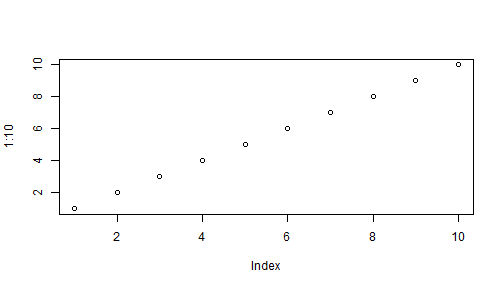
\includegraphics{figs/test/unnamed-chunk-2-1.png}
\caption{plot of chunk unnamed-chunk-2}
\end{figure}


\chapter{Algorithms}
\section{Review of Numerical Methods for Non-Linear Optimizations in Statistics and Related Fields}
\section{Algorithms for Robust Estimators in Statistics}
\section{Propositions}
\subsection{Newton Raphson Algorithms}\label{newton-raphson-algorithms}

\textcite{Sin09} propose a Newton-Raphson algorithm to solve equations
\ref{eq:rml_beta} and \ref{eq:rml_theta} iteratively. The iterative
equation for $\beta$ is given by: \[
\beta^{(m+1)} = \beta^{(m)} + \left(\mathbf{X}^\top \mathbf{V}^{-1}\mathbf{D}(\beta^{(m)})\mathbf{X}\right)^{-1}\mathbf{X}^\top\mathbf{V}^{-1}\mathbf{U}^{\frac{1}{2}}\psi(\mathbf{r}(\beta^{(m)}))
\] where
$\mathbf{D}(\beta) = \frac{\partial \psi(\mathbf{r})}{\partial \mathbf{r}}$
is a diagonal matrix of the same order as $\mathbf{V}$ with elements \[
D_{jj} =
\begin{cases}
1 \text{ for } |r_j|\leq b\\
0 \text{ else}
\end{cases}
\text{ , } j = 1, \dots, n
\] The iterative equation for $\theta$ can be stated as: \[
\theta^{(m+1)} = \theta^{(m)} - \left( \Phi'(\theta^{(m)}) \right)^{-1} \Phi(\theta^{(m)})
\] where $\Phi'(\theta^m)$ is the derivative of $\Phi(\theta)$ evaluated
at $\theta^{(m)}$. The derivative of $\Phi$ is given by
\cite[p.53]{Sch12}:

\begin{align}
\label{eq:deriv_Phi_theta}
\frac{\partial\Phi}{\partial\theta_l} = 2\frac{\partial}{\partial\theta_l}\left(\psi(\mathbf{r})^\top\mathbf{U}^{\frac{1}{2}}\mathbf{V}^{-1}\right)\frac{\partial\mathbf{V}}{\partial\theta_l}\mathbf{V}^{-1}\mathbf{U}^{\frac{1}{2}}\psi(\mathbf{r}) + \tr\left(\mathbf{V}^{-1}\frac{\partial\mathbf{V}}{\partial\theta_l}\mathbf{V}^{-1}\frac{\partial\mathbf{V}}{\partial\theta_l} K\right)
\end{align}

where \[
\frac{\partial}{\partial\theta_l}\left(\psi(\mathbf{r})^\top\mathbf{U}^{\frac{1}{2}}\mathbf{V}^{-1}\right) = \frac{\partial}{\partial\theta_l}(\psi(\mathbf{r})^\top)\mathbf{U}^\frac{1}{2}\mathbf{V}^{-1} + \psi(\mathbf{r})^\top\frac{\partial}{\partial\theta_l}(\mathbf{U}^\frac{1}{2})\mathbf{V}^{-1} - \psi(\mathbf{r})^\top\mathbf{U}^\frac{1}{2}\mathbf{V}^{-1}\frac{\partial\mathbf{V}}{\partial\theta_l}\mathbf{V}^{-1}.
\] In \textcite{Sch12} adopted this procedure for the Spatial Robust
EBLUP and essentially we will follow the same procedure
\textcite[p.74ff.]{Sch12}. Thus we will directly consider the algorithm
for the Spatio Temporal model introduced earlier. Since the model
considered by \textcite{Sin09} contained a block diagonal variance
structure where all off-diagonals are zero, equation
\ref{eq:deriv_Phi_theta} is valid with respect to the earlier specified
variance parameters $\sigma_1^2$ and $\sigma_2^2$ from the spatio
temporal Fay Herriot model. The derivative of $\Phi$ with respect to
$\rho_1$ and $\rho_2$, however, is different. To adapt the notation, let
$\theta = (\sigma_1^2, \sigma_2^2)$ for which equation
\ref{eq:deriv_Phi_theta} holds. Let $\rho = (\rho_1, \rho_2)$ denote the
vector of correlation parameters as they already have been defined
above. Then the iterative equation for $\rho$ is can be stated as: \[
\rho^{(m+1)} = \rho^{(m)} + \left(\Phi'(\rho^{(m)}\right)^{-1}\Phi(\rho^{(m)})
\] where the derivative of $\Phi$ with respect to $\rho$ is given by
\textcite[p.76]{Sch12}:

\begin{align*}
\frac{\partial\Phi}{\partial\rho_l} =& 2\frac{\partial}{\partial\rho_l}\left(\psi(\mathbf{r})^\top\mathbf{U}^{\frac{1}{2}}\mathbf{V}^{-1}\right)\frac{\partial\mathbf{V}}{\partial\rho_l}\mathbf{V}^{-1}\mathbf{U}^{\frac{1}{2}}\psi(\mathbf{r})\\
&+ \psi(\mathbf{r})^\top\mathbf{U}^{\frac{1}{2}}\mathbf{V}^{-1} \frac{\partial\mathbf{V}}{\partial\rho_l\partial\rho_l} \mathbf{V}^{-1}\mathbf{U}^{\frac{1}{2}}\psi(\mathbf{r}) \\
&+ \tr\left(\mathbf{V}^{-1}\frac{\partial\mathbf{V}}{\partial\rho_l\partial\rho_l} K - \mathbf{V}^{-1}\frac{\partial\mathbf{V}}{\partial\theta_l}\mathbf{V}^{-1}\frac{\partial\mathbf{V}}{\partial\theta_l} K\right)
\end{align*}

The partial derivatives of $\mathbf{V}$ with respect to $\theta$ and
$\rho$ are given by:

\begin{align*}
\frac{\partial\mathbf{V}}{\partial\sigma_1^2} =& \mathbf{Z}_1\Omega_1(\rho_1)\mathbf{Z}_1^\top \\
\frac{\partial\mathbf{V}}{\partial\sigma_2^2} =& \Omega_2(\rho_2) \\
\frac{\partial\mathbf{V}}{\partial\rho_1} =& -\sigma_1^2\mathbf{Z}_1\Omega_1(\rho_1)\frac{\partial\Omega_1^{-1}(\rho_1)}{\partial\rho_1}\Omega_1(\rho_1)\mathbf{Z}^\top_1 \\
\frac{\partial\mathbf{V}}{\partial\rho_2} =& \sigma_2^2 \diag\left(\frac{\partial\Omega_{2d}(\rho_2)}{\partial\rho_2}\right) \\
\frac{\partial\mathbf{V}}{\partial\rho_1\partial\rho_1} =& -\sigma_1^2\mathbf{Z}_1\frac{\partial\Omega_1(\rho_1)}{\partial\rho_1}\frac{\partial\Omega_1^{-1}(\rho_1)}{\partial\rho_1}\Omega_1(\rho_1)\mathbf{Z}^\top_1 \\
&-\sigma_1^2\mathbf{Z}_1\Omega_1(\rho_1)\frac{\partial\Omega_1^{-1}(\rho_1)}{\partial\rho_1\partial\rho_1}\Omega_1(\rho_1)\mathbf{Z}^\top_1 \\
&-\sigma_1^2\mathbf{Z}_1\Omega_1(\rho_1)\frac{\partial\Omega_1^{-1}(\rho_1)}{\partial\rho_1}\frac{\partial\Omega_1(\rho_1)}{\partial\rho_1}\mathbf{Z}^\top_1 \\
\frac{\partial\mathbf{V}}{\partial\rho_2\partial\rho_2} =& \text{Needs to be TEXed}
\end{align*}

where

\begin{align*}
\frac{\Omega_1(\rho_1)}{\partial\rho_1} =& -\Omega_1(\rho_1)\frac{\partial\Omega_1^{-1}(\rho_1)}{\partial\rho_1}\Omega_1(\rho_1) \text{ , }\\
\frac{\partial\Omega_1^{-1}(\rho_1)}{\partial\rho_1} =& -\mathbf{W} - \mathbf{W}^\top + 2\rho_1\mathbf{W}^\top\mathbf{W} \text{ , } \\
\frac{\partial\Omega_1^{-1}(\rho_1)}{\partial\rho_1\partial\rho_1} =& 2\mathbf{W}^\top\mathbf{W}\\
\frac{\partial\Omega_{2d}(\rho_2)}{\partial\rho_2} =& \frac{1}{1-\rho_2^2}
\left(
\begin{matrix}
0 & 1 & \cdots & \cdots & (T-1)\rho_2^{T-2}\\
1 & 0 & & & (T-2)\rho_2^{T-3} \\
\vdots & & \ddots & & \vdots \\
(T-2)\rho_2^{T-3} &&& 0 & 1 \\
(T-1)\rho_2^{T-2} & \cdots & \cdots & 1 & 0\\
\end{matrix}
\right) + \frac{2\rho_2\Omega_{2d}(\rho_2)}{1-\rho_2^2}
\end{align*}

Having identified all iterative equations the adapted algorithm from
\textcite{Sch12} is as follows:

\begin{itemize}
\itemsep1pt\parskip0pt\parsep0pt
\item
  Choose initial values for $\beta^0$, $\theta^0$ and $\rho^0$.
\item
  Compute $\beta^{(m+1)}$, with given variance parameters and
  correlation parameters

  \begin{itemize}
  \itemsep1pt\parskip0pt\parsep0pt
  \item
    Compute $\theta^{(m+1)}$, with given regression and correlation
    parameters
  \item
    Compute $\rho^{(m+1)}$, with given variance and regression
    parameters
  \end{itemize}
\item
  Continue step 2 until the following stopping rule holds:
\end{itemize}

\begin{align*}
    ||\beta^{(m+1)}- \beta^{(m)}||^2 <& \text{const} \\
    (\sigma_1^{2(m+1)} - \sigma_1^{2(m)})^2 + (\sigma_2^{2(m+1)} - \sigma_2^{2(m)})^2 + (\rho_1^{(m+1)} - \rho_1^{(m)})^2 + (\rho_2^{(m+1)} - \rho_2^{(m)})^2 <& \text{const}
\end{align*}

\subsection{Fixed Point Algorithms}\label{fixed-point-algorithms}

Inspired by: Chatrchi Golshid (2012): Robust Estimation of Variance
Components in Small Area Estimation, Master-Thesis, Ottawa, Ontario,
Canada: p.~16ff.:

\begin{quote}
The fixed-point iterative method relies on the fixed-point theorem:
"If g(x) is a continuous function for all $x \in [a; b]$, then $g$ has a fixed
point in $[a; b]$." This can be proven by assuming that $g(a)\geq a$ and
$g(b)\leq b$. Since $g$ is continuous the intermediate value theorem guarantees
that there exists a $c$ such that $g(c) = c$.
\end{quote}

Starting from equation \ref{eq:rml_theta} where
$\theta = (\sigma_1^2, \sigma_2^2)$ and $(\rho_1, \rho_2)$ are assumed
to be known, we can rewrite the equation such that:

\begin{align}
\label{eq:rml_theta_fp}
\Phi_l(\theta) = \psi(\mathbf{r})^\top\mathbf{U}^{\frac{1}{2}}\mathbf{V}^{-1}\frac{\partial\mathbf{V}}{\partial\theta_l}\mathbf{V}^{-1}\mathbf{U}^{\frac{1}{2}} \psi(\mathbf{r}) - \tr\left(K\mathbf{V}^{-1}\frac{\partial\mathbf{V}}{\partial\theta_l} (\mathbf{Z}\mathbf{V}_u\mathbf{Z}^\top)^{-1} (\mathbf{Z}\mathbf{V}_u\mathbf{Z}^\top)\right) =& 0
\end{align}

Note that because the matrix $\mathbf{V}_e$ is assumed to be known for
the FH model, it can be omitted. Let $\mathbf{0}_{r\times c}$ define a
matrix filled with 0's of dimension $(r \times c)$ than:

\begin{align*}
\mathbf{Z}\mathbf{V}_u\mathbf{Z}^\top =& \mathbf{Z}\left(\begin{matrix}
\sigma_1^2\Omega_1 & \mathbf{0}_{D\times DT}\\
\mathbf{0}_{DT\times D} &  \sigma_2^2\Omega_2
\end{matrix}\right)\mathbf{Z}^\top \\
=& \mathbf{Z}
\left[
\sigma_1^2\left(\begin{matrix}
\Omega_1 & \mathbf{0}_{D\times DT} \\
\mathbf{0}_{DT\times D} &  \mathbf{0}_{DT\times DT}
\end{matrix}\right) + 
\sigma_2^2\left(\begin{matrix}
\mathbf{0}_{D\times D} & \mathbf{0}_{D\times DT} \\
\mathbf{0}_{DT\times D} & \Omega_2
\end{matrix}\right)
\right]\mathbf{Z}^\top \\
=& \left(\begin{matrix}\mathbf{Z}\bar{\Omega}_1\mathbf{Z}^\top & \mathbf{Z}\bar{\Omega}_2\mathbf{Z}^\top\end{matrix}\right)
\left(\begin{matrix}
\sigma_1^2 \\
\sigma_2^2
\end{matrix}\right)
\end{align*}

Thus equation \ref{eq:rml_theta_fp} can be rewritten to:

\begin{align*}
\psi(\mathbf{r})^\top\mathbf{U}^{\frac{1}{2}}\mathbf{V}^{-1}\frac{\partial\mathbf{V}}{\partial\theta_l}\mathbf{V}^{-1}\mathbf{U}^{\frac{1}{2}} \psi(\mathbf{r}) = \tr\left(K\mathbf{V}^{-1}\frac{\partial\mathbf{V}}{\partial\theta_l} (\mathbf{Z}\mathbf{V}_u\mathbf{Z}^\top)^{-1} \left(\begin{matrix}\mathbf{Z}\bar{\Omega}_1\mathbf{Z}^\top & \mathbf{Z}\bar{\Omega}_2\mathbf{Z}^\top\end{matrix}\right)\left(\begin{matrix}
\sigma_1^2 \\
\sigma_2^2
\end{matrix}\right)\right)
\end{align*}

Let \[
\left(\begin{matrix}
\psi(\mathbf{r})^\top\mathbf{U}^{\frac{1}{2}}\mathbf{V}^{-1}\frac{\partial\mathbf{V}}{\partial\sigma_1^2}\mathbf{V}^{-1}\mathbf{U}^{\frac{1}{2}} \psi(\mathbf{r}) \\
\psi(\mathbf{r})^\top\mathbf{U}^{\frac{1}{2}}\mathbf{V}^{-1}\frac{\partial\mathbf{V}}{\partial\sigma_2^2}\mathbf{V}^{-1}\mathbf{U}^{\frac{1}{2}} \psi(\mathbf{r})
\end{matrix}\right)
= a(\theta) \text{ ,}
\] then \[
\theta = \left(\begin{matrix}
\sigma_1^2 \\
\sigma_2^2
\end{matrix}\right) = A(\theta)^{-1} a(\theta) \text{ ,}
\] where

\begin{align*}
A(\theta) = \left(\begin{matrix}
\tr\left(K\mathbf{V}^{-1}\frac{\partial\mathbf{V}}{\partial\sigma_1^2} (\mathbf{Z}\mathbf{V}_u\mathbf{Z}^\top)^{-1} \mathbf{Z}\bar{\Omega}_1\mathbf{Z}^\top \right) &
\tr\left(K\mathbf{V}^{-1}\frac{\partial\mathbf{V}}{\partial\sigma_1^2} (\mathbf{Z}\mathbf{V}_u\mathbf{Z}^\top)^{-1} \mathbf{Z}\bar{\Omega}_2\mathbf{Z}^\top \right) \\
\tr\left(K\mathbf{V}^{-1}\frac{\partial\mathbf{V}}{\partial\sigma_2^2} (\mathbf{Z}\mathbf{V}_u\mathbf{Z}^\top)^{-1} \mathbf{Z}\bar{\Omega}_1\mathbf{Z}^\top \right) &
\tr\left(K\mathbf{V}^{-1}\frac{\partial\mathbf{V}}{\partial\sigma_2^2} (\mathbf{Z}\mathbf{V}_u\mathbf{Z}^\top)^{-1} \mathbf{Z}\bar{\Omega}_2\mathbf{Z}^\top \right)
\end{matrix}\right) \text{.}
\end{align*}

So, the fixed point algorithm can be presented as follows: \[
\theta^{m+1} = A(\theta^{(m)})^{-1} a(\theta^{(m)})
\]

At this time the fixed-point algorithm for
$\theta = (\sigma_1^2, \sigma_2^2)$ will replace the corresponding step
in Issue 1.

\subsubsection{N-S: Fixed-Point-Algorithm - Spatial
Correlation}\label{n-s-fixed-point-algorithm---spatial-correlation}

To extend the above algorithm to not only being used for the estimation
of $\theta = (\sigma_1^2, \sigma_2^2)$ but also for the spatial
correlation parameter $\rho_1$ reconsider:

\begin{eqnarray}
\label{eq:zVuZ_rho1_1}
\mathbf{Z}\mathbf{V}_u\mathbf{Z}^\top &=& \mathbf{Z}\left(\begin{matrix}
\sigma_1^2\Omega_1 & \mathbf{0}_{D\times DT}\\
\mathbf{0}_{DT\times D} &  \sigma_2^2\Omega_2
\end{matrix}\right)\mathbf{Z}^\top
\end{eqnarray}

and the specification of
$\Omega_1(\rho_1) = \left((I-\rho_1\mathbf{W})^\top(I-\rho_1\mathbf{W})\right)^{-1}$:

\begin{align}
\sigma_1^2\Omega_1(\rho_1) &= \sigma_1^2\Omega_1\Omega_1(I-\rho_1\mathbf{W})^\top(I-\rho_1\mathbf{W}) \notag\\
&= \sigma_1^2\left(\Omega_1\Omega_1 -\rho_1\Omega_1\Omega_1\mathbf{W}^\top -\rho_1\Omega_1\Omega_1\mathbf{W} + \rho_1^2\Omega_1\Omega_1\mathbf{W}^\top\mathbf{W}\right) \notag\\
&= \sigma_1^2\left(\Omega_1\Omega_1 -\rho_1\Omega_1\Omega_1\mathbf{W}^\top\right) +\rho_1 \left(-\sigma_1^2\Omega_1\Omega_1\mathbf{W} + \sigma_1^2\rho_1\Omega_1\Omega_1\mathbf{W}^\top\mathbf{W}\right) \label{eq:zVuZ_rho1_2}
\end{align}

Thus equation \ref{eq:zVuZ_rho1_1} can be rewritten as:

\begin{align*}
\mathbf{Z}\mathbf{V}_u\mathbf{Z}^\top
&=\mathbf{Z}
\Biggr[
\sigma_1^2\left(\begin{matrix}
\Omega_1\Omega_1 -\rho_1\Omega_1\Omega_1\mathbf{W}^\top & \mathbf{0}_{D\times DT}\\
\mathbf{0}_{DT\times D} &  \mathbf{0}_{DT\times DT}
\end{matrix}\right)\\
&+\rho_1\left(\begin{matrix}
-\sigma_1^2\Omega_1\Omega_1\mathbf{W} + \sigma_1^2\rho_1\Omega_1\Omega_1\mathbf{W}^\top\mathbf{W} & \mathbf{0}_{D\times DT}\\
\mathbf{0}_{DT\times D} &  \mathbf{0}_{DT\times DT}
\end{matrix}\right)\\
&+\sigma_2^2\left(\begin{matrix}
\mathbf{0}_{D\times D} & \mathbf{0}_{D\times DT}\\
\mathbf{0}_{DT\times D} & \Omega_2
\end{matrix}\right)
\Biggr]
\mathbf{Z}^\top \\
&=\left(\begin{matrix}\mathbf{Z}\bar{\Omega}_{1, \sigma_1^2}\mathbf{Z}^\top & 
\mathbf{Z}\bar{\Omega}_{1, \rho_1}\mathbf{Z}^\top & \mathbf{Z}\bar{\Omega}_2\mathbf{Z}^\top\end{matrix}\right)
\left(\begin{matrix}
\sigma_1^2 \\
\rho_1 \\
\sigma_2^2
\end{matrix}\right)
\end{align*}

Thus equation \ref{eq:rml_theta_fp} can be rewritten (analogously as
above) to:

\begin{eqnarray*}
\psi(\mathbf{r})^\top\mathbf{U}^{\frac{1}{2}}\mathbf{V}^{-1}\frac{\partial\mathbf{V}}{\partial\theta_l}\mathbf{V}^{-1}\mathbf{U}^{\frac{1}{2}} \psi(\mathbf{r}) = \tr\left(K\mathbf{V}^{-1}\frac{\partial\mathbf{V}}{\partial\theta_l} (\mathbf{Z}\mathbf{V}_u\mathbf{Z}^\top)^{-1} \left(\begin{matrix}\mathbf{Z}\bar{\Omega}_{1, \sigma_1^2}\mathbf{Z}^\top & 
\mathbf{Z}\bar{\Omega}_{1, \rho_1}\mathbf{Z}^\top & \mathbf{Z}\bar{\Omega}_2\mathbf{Z}^\top\end{matrix}\right)
\left(\begin{matrix}
\sigma_1^2 \\
\rho_1 \\
\sigma_2^2
\end{matrix}\right)\right)
\end{eqnarray*}

Let

\[
\left(\begin{matrix}
\psi(\mathbf{r})^\top\mathbf{U}^{\frac{1}{2}}\mathbf{V}^{-1}\frac{\partial\mathbf{V}}{\partial\sigma_1^2}\mathbf{V}^{-1}\mathbf{U}^{\frac{1}{2}} \psi(\mathbf{r}) \\
\psi(\mathbf{r})^\top\mathbf{U}^{\frac{1}{2}}\mathbf{V}^{-1}\frac{\partial\mathbf{V}}{\partial\rho_1}\mathbf{V}^{-1}\mathbf{U}^{\frac{1}{2}} \psi(\mathbf{r}) \\
\psi(\mathbf{r})^\top\mathbf{U}^{\frac{1}{2}}\mathbf{V}^{-1}\frac{\partial\mathbf{V}}{\partial\sigma_2^2}\mathbf{V}^{-1}\mathbf{U}^{\frac{1}{2}} \psi(\mathbf{r})
\end{matrix}\right)
= a(\theta) \text{ ,}
\]

then

\[
\theta = \left(\begin{matrix}
\sigma_1^2 \\
\rho_1 \\
\sigma_2^2
\end{matrix}\right) = A(\theta)^{-1} a(\theta) \text{ ,}
\] where

\begin{align*}
A(\theta) = \left(\begin{matrix}
\tr\left(\gamma(\sigma_1^2) \mathbf{Z}\bar{\Omega}_{1,\sigma_1^2} \mathbf{Z}^\top \right) & \tr\left(\gamma(\sigma_1^2) \mathbf{Z}\bar{\Omega}_{1,\rho_1} \mathbf{Z}^\top \right) &
\tr\left(\gamma(\sigma_1^2) \mathbf{Z}\bar{\Omega}_2\mathbf{Z}^\top \right) \\
\tr\left(\gamma(\rho_1) \mathbf{Z}\bar{\Omega}_{1,\sigma_1^2} \mathbf{Z}^\top \right) & \tr\left(\gamma(\rho_1) \mathbf{Z}\bar{\Omega}_{1,\rho_1} \mathbf{Z}^\top \right) &
\tr\left(\gamma(\rho_1) \mathbf{Z}\bar{\Omega}_2\mathbf{Z}^\top \right) \\
\tr\left(\gamma(\sigma_2^2) \mathbf{Z}\bar{\Omega}_{1,\sigma_1^2} \mathbf{Z}^\top \right) & \tr\left(\gamma(\sigma_2^2) \mathbf{Z}\bar{\Omega}_{1,\rho_1} \mathbf{Z}^\top \right) &
\tr\left(\gamma(\sigma_2^2) \mathbf{Z}\bar{\Omega}_2\mathbf{Z}^\top \right)
\end{matrix}\right)
\end{align*}

and
$\gamma(\theta_l) = K\mathbf{V}^{-1}\frac{\partial\mathbf{V}}{\partial\theta_l} (\mathbf{Z}\mathbf{V}_u\mathbf{Z}^\top)^{-1}$

\subsubsection{More on the Fixed Point}\label{more-on-the-fixed-point}

Inspired by: Chatrchi Golshid (2012): Robust Estimation of Variance
Components in Small Area Estimation, Master-Thesis, Ottawa, Ontario,
Canada: p.~16ff.:

\begin{quote}
The fixed-point iterative method relies on the fixed-point theorem: "If g(x) is
a continuous function for all $x \in [a; b]$, then $g$ has a fixed point in $[a;
b]$." This can be proven by assuming that $g(a)\geq a$ and $g(b)\leq b$. Since
$g$ is continuous the intermediate value theorem guarantees that there exists a
$c$ such that $g(c) = c$.
\end{quote}

Starting from equation \ref{eq:rml_theta} where
$\theta = \randomEffectVariance$ we can rewrite the equation such that:

\begin{align}
\label{eq:rml_theta_fp}
\Phi(\theta) = \aFH - \tr\left(K\mathbf{V}^{-1}\frac{\partial\mathbf{V}}{\partial\theta} (\mathbf{Z}\mathbf{G}\mathbf{Z}^\top)^{-1} (\mathbf{Z}\mathbf{G}\mathbf{Z}^\top)\right) =& 0
\end{align}

Note that because the matrix $\mathbf{R}$ is assumed to be known for the
FH model, it can be omitted. Note that under the simple Fay-Herriot
Model
$\mathbf{Z}\mathbf{G}\mathbf{Z}^\top = \randomEffectVariance\IdentityMatrix$,
where $\IdentityMatrix$ is a $(\nDomains \times \nDomains)$ identity
matrix. Furthermore
$\frac{\partial\mathbf{V}}{\partial\theta} = \IdentityMatrix$. Thus
equation \ref{eq:rml_theta_fp} can be rewritten to:

\begin{align*}
\psi(\mathbf{r})^\top\mathbf{U}^{\frac{1}{2}}\mathbf{V}^{-1}\mathbf{V}^{-1}\mathbf{U}^{\frac{1}{2}} \psi(\mathbf{r}) = \tr\left(K\mathbf{V}^{-1}\mathbf{G}^{-1} \randomEffectVariance \right)
\end{align*}

This can be solved for the fixed Point and is directly presented in
algorithmic notation, such that: \[
\theta^{m+1} = A(\theta^{(m)})^{-1} a(\theta^{(m)}) \text{ ,}
\] where \[
A(\theta) = \tr\left(K\mathbf{V}^{-1}\mathbf{G}^{-1} \right)
\] and
\[a(\theta) = \psi(\mathbf{r})^\top\mathbf{U}^{\frac{1}{2}}\mathbf{V}^{-1}\mathbf{V}^{-1}\mathbf{U}^{\frac{1}{2}} \psi(\mathbf{r})
\]


%------------------------------------------------

\ctparttext{This is the part where I want to introduce the software where the theoretical concepts find implementation.}

\part{Implementation}
\chapter{Verification of Results}
\chapter{Performance of Algorithms, a Statisticians Perspective}
\chapter{Validation of Point Estimates, a Users Perspective}
\chapter{Software}

%------------------------------------------------

\ctparttext{This is the part where I will present all results. Most certainly they will contain a lot of model- and design-based simulation studies for various settings. Maybe there will be more data available and I can present some applications.}

\part{Results}
\chapter{Numerical Accuracy}
\chapter{Stability}
\chapter{Speed of Convergence}
\chapter{Computational Complexity}
\chapter{Simulation Studies}
\section{Area Level Models}
\subsection{The Area-Level Perspective}
\input{Rmd/results_area_level_mc}

\subsection{From Unit to Area Level Data}
\input{Rmd/results_unit_to_area_level_mc}

%----------------------------------------------------------------------------------------
%	THESIS CONTENT - APPENDICES
%----------------------------------------------------------------------------------------

\appendix

\part{Appendix} % New part of the thesis for the appendix

%\include{Chapters/Chapter0A} % Appendix A
%\include{Chapters/Chapter0B} % Appendix B - empty template

%----------------------------------------------------------------------------------------
%	POST-CONTENT THESIS PAGES
%----------------------------------------------------------------------------------------

\cleardoublepage% Bibliography

\label{app:bibliography} % Reference the bibliography elsewhere with \autoref{app:bibliography}

\manualmark
\markboth{\spacedlowsmallcaps{\bibname}}{\spacedlowsmallcaps{\bibname}} 
\refstepcounter{dummy}

\addtocontents{toc}{\protect\vspace{\beforebibskip}} % Place the bibliography slightly below the rest of the document content in the table of contents
\addcontentsline{toc}{chapter}{\tocEntry{\bibname}}

\printbibliography % Bibliography

%\cleardoublepage% Colophon (a brief description of publication or production notes relevant to the edition)

\pagestyle{empty}

\hfill

\vfill

\pdfbookmark[0]{Colophon}{colophon}

\section*{Colophon}

This document was typeset using the typographical look-and-feel \texttt{classicthesis} developed by Andr\'e Miede. The style was inspired by Robert Bringhurst's seminal book on typography ``\emph{The Elements of Typographic Style}''. \texttt{classicthesis} is available for both \LaTeX\ and \mLyX: 

\begin{center}
\url{http://code.google.com/p/classicthesis/}
\end{center}

\noindent Happy users of \texttt{classicthesis} usually send a real postcard to the author, a collection of postcards received so far is featured here: 

\begin{center}
\url{http://postcards.miede.de/}
\end{center}
 
\bigskip

\noindent\finalVersionString % Colophon

%\cleardoublepage% Declaration

\refstepcounter{dummy}
\pdfbookmark[0]{Declaration}{declaration} % Bookmark name visible in a PDF viewer

\chapter*{Declaration} % Declaration section text

\thispagestyle{empty}

Put your declaration here.
\bigskip
 
\noindent\textit{\myLocation, \myTime}

\smallskip

\begin{flushright}
\begin{tabular}{m{5cm}}
\\ \hline
\centering\myName, \today \\
\end{tabular}
\end{flushright}
 % Declaration

%----------------------------------------------------------------------------------------

\end{document}
